\chapter{Metodologia}
\label{chap:metodologia}

O HoTHP (\textit{Hyperbolic Rotary Position Embedding-based Transformer Hawkes Process}) é uma variante do THP que substitui o kernel trigonométrico do RoTHP por um kernel hiperbólico com decaimento exponencial, inspirado no HoPE \cite{dai_hope_2025}. A principal motivação é a extrapolação de comprimento, onde treinamos em sequências curtas e mantemos o desempenho estável em sequências mais longas. O mecanismo por trás dessa capacidade é um viés exponencial de recência embutido diretamente no kernel de atenção, que faz os scores decaírem monotonicamente com a distância temporal, refletindo a estrutura do próprio processo de Hawkes.

% ---------------------------------------------------------------
\section{A limitação oscilatória do RoTHP}
\label{sec:limitacao-rothp}
% ---------------------------------------------------------------

Como vimos na Seção \ref{sec:processos-de-hawkes-utilizando-transformers}, o RoTHP representa a posição de cada evento por uma rotação trigonométrica aplicada aos vetores de query $\mathbf{q}$ e key $\mathbf{k}$. O score de atenção entre os eventos $i$ e $j$ depende apenas de $\Delta t = t_i - t_j$, o que é garantido pelas propriedades algébricas das matrizes de rotação.

O problema é que o kernel resultante é oscilatório. Seno e cosseno não são funções monótonas. Sendo assim, o score de atenção pode crescer para eventos mais distantes no tempo, dependendo da fase da oscilação, e diminuir para eventos próximos. Isso contradiz diretamente o kernel de influência do processo de Hawkes, $\varphi(\Delta t) = \alpha e^{-\beta \Delta t}$, que é estritamente decrescente.

Na prática, a consequência mais grave dessa oscilação aparece na extrapolação de comprimento. Quando testado em sequências mais longas do que as de treinamento, o modelo encontra diferenças temporais $\Delta t$ que nunca observou durante o treino. Um kernel com decaimento exponencial teria um comportamento previsível nessa região, com a influência continuando a cair. Já o kernel trigonométrico continua oscilando com a mesma amplitude, e um evento muito distante pode receber um score alto simplesmente porque a fase do cosseno calhou num pico naquele $\Delta t$. O modelo não aprendeu a lidar com essas fases porque nunca as viu durante o treino, e o kernel não tem nada que force o score a decair. É essa ausência de viés de recência que impede o RoTHP de extrapolar de forma estável.

% ---------------------------------------------------------------
\section{Do kernel trigonométrico ao kernel hiperbólico}
\label{sec:trig-to-hyp}
% ---------------------------------------------------------------

Para cada par de dimensões $(2j{-}1, 2j)$, o RoTHP aplica o bloco $2 \times 2$ de rotação trigonométrica:
%
\begin{equation}
    \boldsymbol{R}_j(\Delta t) = \begin{bmatrix} \cos(\theta_j \Delta t) & \sin(\theta_j \Delta t) \\ -\sin(\theta_j \Delta t) & \cos(\theta_j \Delta t) \end{bmatrix}.
\end{equation}
%
O HoPE \cite{dai_hope_2025} propõe trocar essa rotação por uma rotação hiperbólica, cujo bloco correspondente é:
%
\begin{equation}
    \boldsymbol{B}_j(\Delta t) = \begin{bmatrix} \cosh(\theta_j \Delta t) & \sinh(\theta_j \Delta t) \\ \sinh(\theta_j \Delta t) & \cosh(\theta_j \Delta t) \end{bmatrix}.
    \label{eq:bloco-hiperbolico}
\end{equation}
%
Diferentemente de $\cos$ e $\sin$, as funções $\cosh$ e $\sinh$ são monótonas para $\Delta t > 0$, eliminando as oscilações. Entretanto, não podemos usar $\boldsymbol{B}_j$ diretamente porque a rotação hiperbólica não é ortogonal, e o produto interno $\boldsymbol{q}^\top \boldsymbol{B}(\Delta t) \boldsymbol{k}$ \textit{cresce} com $|\Delta t|$ em vez de decair \cite{dai_hope_2025}. Eventos distantes receberiam scores maiores do que eventos próximos, exatamente o oposto do que queremos.

A Figura~\ref{fig:trig-vs-hyp} ilustra essa diferença. No painel esquerdo, $\cos$ e $\sin$ oscilam entre $-1$ e $1$ indefinidamente, sem qualquer tendência de decaimento. No painel direito, $\cosh$ e $\sinh$ eliminam as oscilações mas crescem exponencialmente em ambas as direções. Note que $\cosh$ é uma função par (simétrica, com valor mínimo $\cosh(0) = 1$) enquanto $\sinh$ é ímpar (antissimétrica, com $\sinh(0) = 0$). Para $\Delta t$ grande, ambas se aproximam de $\frac{e^{\theta|\Delta t|}}{2}$.

\begin{figure}[h!]
    \centering
    \captionsetup{width=14cm}
    \Caption{\label{fig:trig-vs-hyp} Funções base dos kernels de atenção ($\theta = 1{,}0$). Esquerda: funções trigonométricas do RoTHP, que oscilam entre $-1$ e $1$ sem decair. Direita: funções hiperbólicas do HoPE, que são monótonas mas crescem exponencialmente. O crescimento das funções hiperbólicas precisa ser compensado por um fator de decaimento para que o kernel de atenção funcione corretamente.}
    \UFCfig{}{
        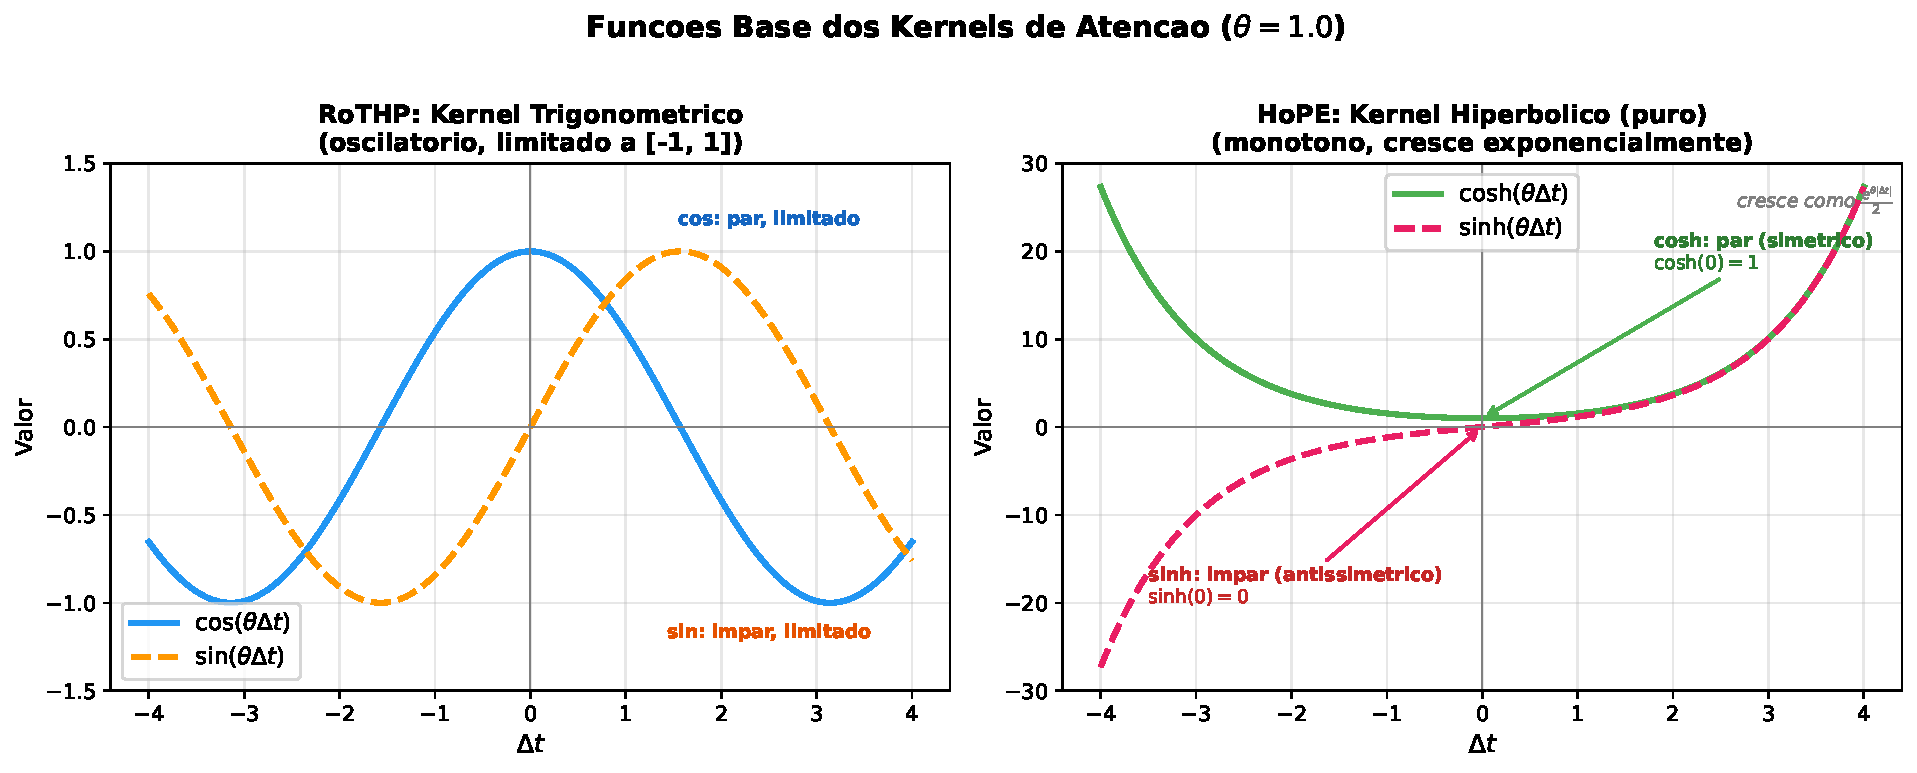
\includegraphics[width=14cm]{figuras/fig_trig_vs_hyp.pdf}
    }{
    }
\end{figure}

% ---------------------------------------------------------------
\section{Decaimento exponencial e o parâmetro \texorpdfstring{$\theta'$}{theta'}}
\label{sec:decaimento-theta-prime}
% ---------------------------------------------------------------

Para corrigir o crescimento hiperbólico, o HoPE \cite{dai_hope_2025} introduz um parâmetro aprendível $\theta'$ e aplica fatores de amortecimento nos vetores $\boldsymbol{q}$ e $\boldsymbol{k}$. O vetor $\boldsymbol{q}$ na posição $m$ é multiplicado por $e^{-m\theta'}$, e o vetor $\boldsymbol{k}$ na posição $n$ é multiplicado por $e^{+n\theta'}$. Ao computar o score entre as posições $m$ e $n$, esses fatores se combinam:
%
\begin{equation}
    g(\boldsymbol{x}_m, \boldsymbol{x}_n, m{-}n) = e^{-(m-n)\theta'} \; \boldsymbol{q}^\top \boldsymbol{B}(\theta, m{-}n) \; \boldsymbol{k}.
    \label{eq:hope-score-discreto}
\end{equation}
%
No HoTHP, as posições discretas $m, n$ são substituídas pelos instantes contínuos $t_i, t_j$, e a diferença $m - n$ pela diferença temporal $\Delta t = t_i - t_j$:
%
\begin{equation}
    g(\Delta t) = e^{-\Delta t \cdot \theta'} \; \boldsymbol{q}^\top \, \boldsymbol{B}(\theta, \Delta t) \; \boldsymbol{k}.
    \label{eq:kernel-hothp-completo}
\end{equation}
%
Para que o decaimento domine o crescimento hiperbólico, é necessário que $\theta' > \max_j \theta_j$. Sob essa condição, o score decresce monotonicamente com $|\Delta t|$, o que introduz um viés exponencial de recência no mecanismo de atenção. Esse viés reflete a mesma estrutura do kernel de Hawkes ($\alpha e^{-\beta \Delta t}$) e, por ser estrutural e não aprendido dos dados, vale inclusive para valores de $\Delta t$ que o modelo nunca viu durante o treinamento. É esse viés que dá ao HoTHP a capacidade de extrapolar para sequências mais longas sem degradação.

A Figura~\ref{fig:decay-hiperbolico} ilustra esse mecanismo. O painel esquerdo mostra os componentes separados: $\cosh$ e $\sinh$ crescem exponencialmente enquanto o fator de decaimento $e^{-\theta'\Delta t}$ cai rapidamente para zero. O painel central mostra o produto: quando $\theta' > \theta$, o decaimento domina o crescimento, e tanto $e^{-\theta'\Delta t}\cosh(\theta\Delta t)$ quanto $e^{-\theta'\Delta t}\sinh(\theta\Delta t)$ decaem monotonicamente. O painel direito mostra a decomposição em exponenciais puras usada na implementação (Seção~\ref{sec:estabilidade-numerica}): como ambos os expoentes $(\theta' - \theta)$ e $(\theta' + \theta)$ são positivos, todas as exponenciais têm argumento negativo e nenhum overflow ocorre.

\begin{figure}[h!]
    \centering
    \captionsetup{width=14cm}
    \Caption{\label{fig:decay-hiperbolico} Efeito do decaimento exponencial sobre as funções hiperbólicas ($\theta = 1{,}0$, $\theta' = 1{,}5$). Esquerda: componentes separados, mostrando que $\cosh$ e $\sinh$ crescem mas o decay cai. Centro: o produto resulta em funções que decaem monotonamente. Direita: decomposição em exponenciais puras, ambas com expoente negativo, garantindo estabilidade numérica.}
    \UFCfig{}{
        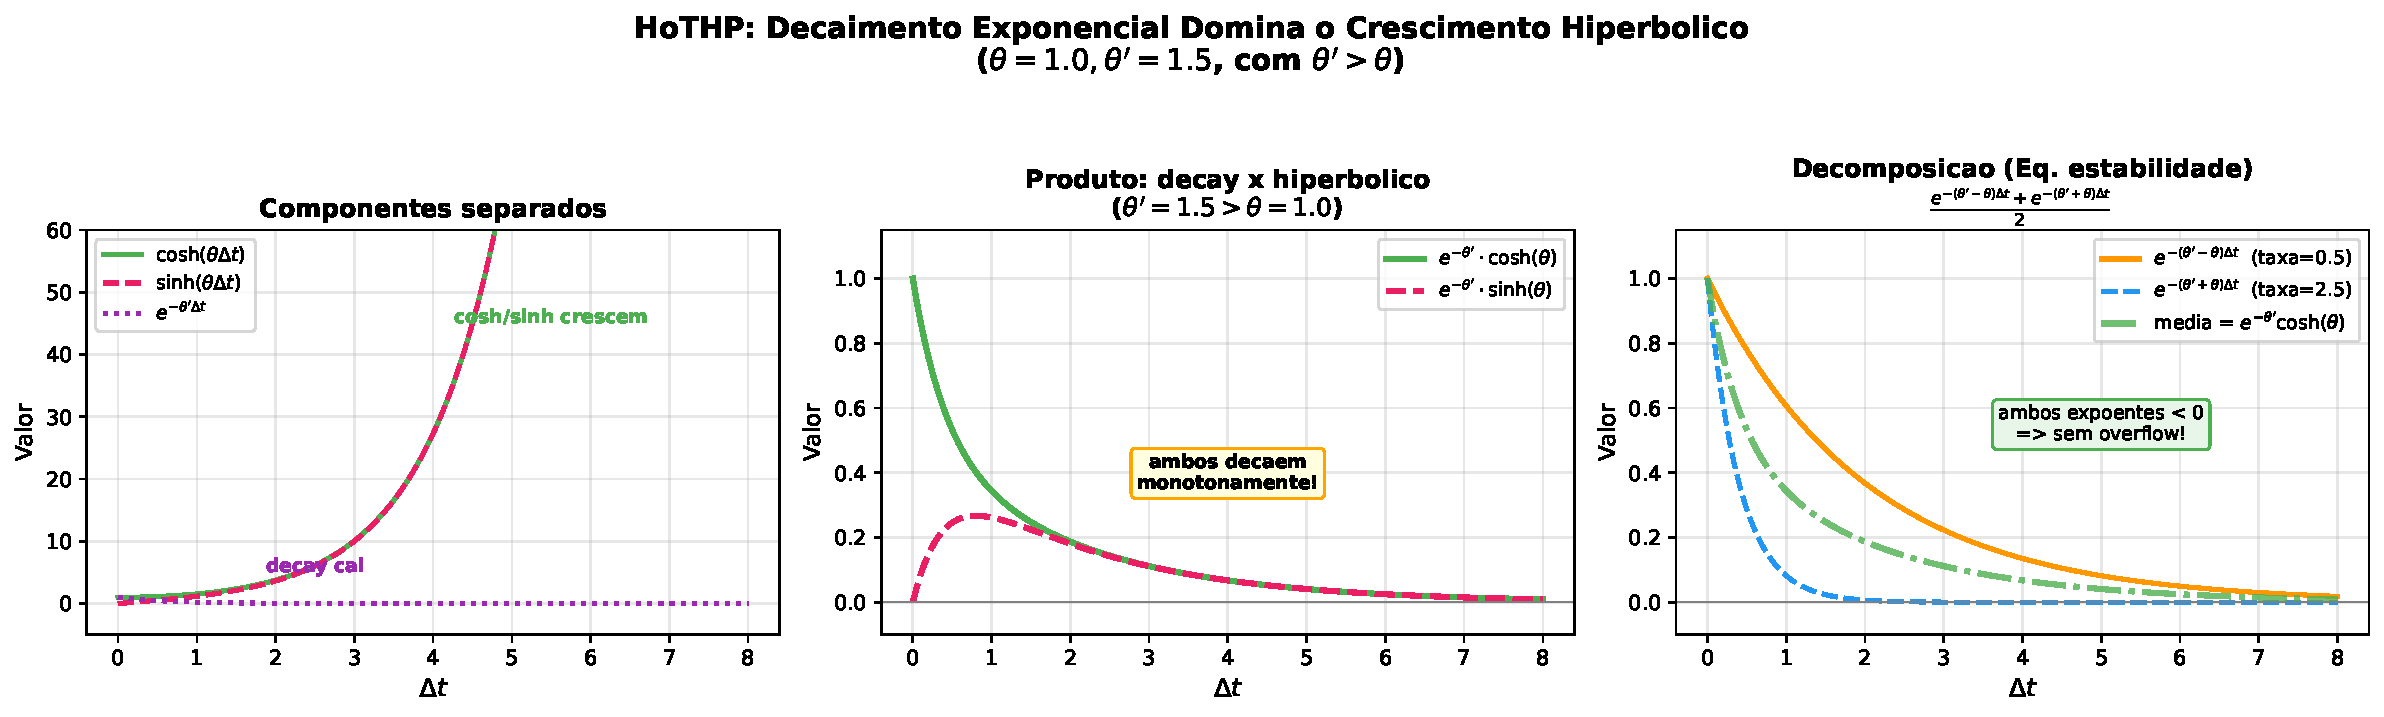
\includegraphics[width=14cm]{figuras/fig_decay_hiperbolico.pdf}
    }{
    }
\end{figure}

\subsection{Parametrização do \texorpdfstring{$\theta'$}{theta'} aprendível}
\label{subsec:parametrizacao-theta-prime}

Como $\theta'$ precisa ser aprendível mas ao mesmo tempo satisfazer $\theta' > \max_j \theta_j$, não podemos simplesmente treinar um parâmetro livre. A solução é parametrizá-lo como:
%
\begin{equation}
    \theta' = \mathrm{softplus}(\theta'_{\mathrm{raw}}) + \max_j(\theta_j) + \epsilon,
    \label{eq:theta-prime-parametrizacao}
\end{equation}
%
onde $\theta'_{\mathrm{raw}}$ é o parâmetro treinável (inicializado em $0{,}5$), $\mathrm{softplus}(x) = \ln(1 + e^x)$ garante que o primeiro termo seja positivo, e $\epsilon = 10^{-4}$ é uma margem de segurança. Assim, $\theta'$ é sempre maior do que qualquer $\theta_j$, e o decaimento exponencial é garantido estruturalmente, independentemente do que o gradiente faça.

As frequências $\theta_j$ seguem a fórmula do RoPE \cite{su_roformer_2023}:
%
\begin{equation}
    \theta_j = 10000^{-2(j-1)/d}, \quad j = 1, \ldots, d/2,
    \label{eq:frequencias-theta}
\end{equation}
%
onde $d$ é a dimensão de cada cabeça de atenção. Cada par de dimensões recebe uma frequência diferente, cobrindo múltiplas escalas de $\Delta t$.

% ---------------------------------------------------------------
\section{Score de atenção do HoTHP}
\label{sec:score-atencao-hothp}
% ---------------------------------------------------------------

Expandindo a multiplicação matricial de $\boldsymbol{B}_j$ (Equação \ref{eq:bloco-hiperbolico}) sobre um par de dimensões $(q_1, q_2)$ e $(k_1, k_2)$, obtemos:
%
\begin{equation}
    \boldsymbol{q}^\top \boldsymbol{B}_j(\Delta t) \boldsymbol{k}
    = \underbrace{(q_1 k_1 + q_2 k_2)}_{\text{parte cosh}} \cdot \cosh(\theta_j \Delta t)
    + \underbrace{(q_1 k_2 + q_2 k_1)}_{\text{parte sinh}} \cdot \sinh(\theta_j \Delta t).
    \label{eq:score-par-dimensoes}
\end{equation}
%
O score completo incorpora o fator de decaimento e soma sobre os $d/2$ pares de dimensões:
%
\begin{equation}
    s_{ij} = \frac{1}{\sqrt{d}} \sum_{j=1}^{d/2}
    \left[
        (q_{1}^{(j)} k_{1}^{(j)} + q_{2}^{(j)} k_{2}^{(j)}) \cdot e^{-|\Delta t|\theta'} \cosh(\theta_j \Delta t)
        + (q_{1}^{(j)} k_{2}^{(j)} + q_{2}^{(j)} k_{1}^{(j)}) \cdot e^{-|\Delta t|\theta'} \sinh(\theta_j \Delta t)
    \right],
    \label{eq:score-hothp-completo}
\end{equation}
%
onde $\Delta t = t_i - t_j$ e $1/\sqrt{d}$ é a normalização padrão do \textit{scaled dot-product attention} \cite{vaswani_attention_2017}.

No RoTHP, os vetores $\boldsymbol{q}$ e $\boldsymbol{k}$ são pré-rotacionados individualmente por $\boldsymbol{R}(t_i)$ e $\boldsymbol{R}(t_j)$ antes do produto interno, e a dependência em $\Delta t$ emerge do cancelamento algébrico. No HoTHP, o score é formulado diretamente em termos de $\Delta t$, o que torna natural incluir o fator $e^{-|\Delta t|\theta'}$ dentro do próprio kernel. A consequência prática é que, para qualquer $\Delta t$ (incluindo valores maiores do que os vistos no treino), o score é dominado pelo decaimento exponencial. Esse é o mecanismo que permite a extrapolação: o viés de recência não depende dos dados, ele está na estrutura da atenção.

% ---------------------------------------------------------------
\section{Estabilidade numérica}
\label{sec:estabilidade-numerica}
% ---------------------------------------------------------------

As funções $\cosh$ e $\sinh$ crescem como $e^{|\Delta t|\theta_j}$, e para eventos muito espaçados esses valores podem causar \textit{overflow} em ponto flutuante antes mesmo de serem multiplicados pelo fator de decaimento $e^{-|\Delta t|\theta'}$.

A solução é distribuir o decaimento para dentro das funções hiperbólicas usando as identidades:
%
\begin{align}
    e^{-|\Delta t|\theta'} \cdot \cosh(|\Delta t|\theta_j)
    &= \frac{e^{-|\Delta t|(\theta' - \theta_j)} + e^{-|\Delta t|(\theta' + \theta_j)}}{2},
    \label{eq:decay-cosh}\\[4pt]
    e^{-|\Delta t|\theta'} \cdot \sinh(\Delta t \cdot \theta_j)
    &= \mathrm{sgn}(\Delta t) \cdot \frac{e^{-|\Delta t|(\theta' - \theta_j)} - e^{-|\Delta t|(\theta' + \theta_j)}}{2}.
    \label{eq:decay-sinh}
\end{align}
%
Como $\theta' > \max_j \theta_j$, temos $\theta' - \theta_j > 0$ e $\theta' + \theta_j > 0$, portanto ambos os expoentes são negativos para qualquer $\Delta t$, e o \textit{overflow} não ocorre. O sinal de $\Delta t$ é reintroduzido explicitamente por $\mathrm{sgn}(\Delta t)$, pois $\sinh(-x) = -\sinh(x)$.

% ---------------------------------------------------------------
\section{Normalização temporal}
\label{sec:normalizacao-temporal}
% ---------------------------------------------------------------

Datasets diferentes têm escalas temporais muito distintas. Em redes sociais, os intervalos entre eventos podem estar na ordem de milissegundos, enquanto em dados sísmicos ficam na ordem de dias. Se usássemos os instantes brutos no kernel hiperbólico, os valores de $\theta_j \Delta t$ estariam em escalas incompatíveis e o modelo precisaria de hiperparâmetros específicos para cada dataset.

Para evitar isso, deslocamos os instantes de cada sequência de modo que ela comece em zero:
%
\begin{equation}
    \tilde{t}_i = t_i - t_1, \quad i = 1, \ldots, N.
    \label{eq:normalizacao-temporal}
\end{equation}
%
Essa operação é feita independentemente para cada sequência no \textit{batch}. As diferenças $\Delta \tilde{t} = \tilde{t}_i - \tilde{t}_j = t_i - t_j$ são preservadas, de modo que os intervalos inter-evento originais não se alteram.

% ---------------------------------------------------------------
\section{Arquitetura completa}
\label{sec:arquitetura-hothp}
% ---------------------------------------------------------------

A arquitetura do HoTHP segue o encoder do Transformer \cite{vaswani_attention_2017}, ilustrada na Figura \ref{fig:arquitetura-hothp}. Cada evento $(t_i, k_i)$ é representado por um embedding de tipo aprendível $\boldsymbol{e}_{k_i} \in \mathbb{R}^d$. Ao contrário do THP \cite{zuo_transformer_2021}, que soma um encoding sinusoidal do tempo absoluto ao embedding, o HoTHP não inclui nenhuma informação temporal no embedding. Os instantes $t_i$ entram no modelo apenas pelo kernel hiperbólico.

\begin{figure}[h!]
    \centering
    \captionsetup{width=14cm}
    \Caption{\label{fig:arquitetura-hothp}Arquitetura do HoTHP. O embedding de tipo é passado por camadas de encoder com atenção hiperbólica. A informação temporal entra exclusivamente pelo kernel hiperbólico, que recebe as diferenças $\Delta t$ normalizadas.}
    \UFCfig{}{
        
\includegraphics[width=14cm]{../overleaf-bracis/figures/architecture.pdf}
    }{
        \Fonte{Elaborado pelo autor.}
    }
\end{figure}

O modelo empilha $N_{\ell}$ camadas de encoder hiperbólico, cada uma com um bloco de atenção multi-cabeça hiperbólica seguido de uma rede \textit{feed-forward}. A atenção computa os scores via Equação \ref{eq:score-hothp-completo}, usando as diferenças normalizadas $\Delta\tilde{t}_{ij} = \tilde{t}_i - \tilde{t}_j$. Uma máscara causal garante que cada evento atenda apenas a eventos anteriores.

A rede \textit{feed-forward} em cada camada tem duas projeções lineares com ReLU entre elas:
%
\begin{equation}
    \mathrm{FFN}(\boldsymbol{x}) = \boldsymbol{W}_2 \cdot \mathrm{ReLU}(\boldsymbol{W}_1 \boldsymbol{x} + \boldsymbol{b}_1) + \boldsymbol{b}_2,
\end{equation}
%
com dimensão interna $2d$. Assim como o RoTHP \cite{gao_rothp_2024}, o HoTHP não usa conexões residuais (add \& norm).

A saída do encoder $\boldsymbol{h}(t_j) \in \mathbb{R}^d$ para o evento $j$ é usada para calcular a intensidade condicional de cada tipo $k$ no instante $t > t_j$:
%
\begin{equation}
    \lambda_k(t \mid \mathcal{H}_t)
    = \mathrm{softplus}\!\left(
        \alpha_k \frac{t - t_j}{t_j + \epsilon}
        + \boldsymbol{w}_k^\top \boldsymbol{h}(t_j)
        + b_k
    \right),
    \label{eq:intensidade-hothp}
\end{equation}
%
onde $\alpha_k$, $\boldsymbol{w}_k$ e $b_k$ são parâmetros aprendíveis e $\mathrm{softplus}$ garante que a intensidade seja positiva. O termo $\alpha_k (t - t_j) / t_j$ captura a variação com o tempo desde o último evento, e $\boldsymbol{w}_k^\top \boldsymbol{h}(t_j)$ traz o contexto histórico do encoder. Essa forma segue o THP \cite{zuo_transformer_2021}.

% ---------------------------------------------------------------
\section{Onde atua o viés exponencial}
\label{sec:onde-atua-vies}
% ---------------------------------------------------------------

Uma distinção importante precisa ser feita sobre o papel do decaimento exponencial no HoTHP. O fator $e^{-|\Delta t|\theta'}$ não atua diretamente na função de intensidade $\lambda_k(t)$, e sim no mecanismo de atenção que produz o estado oculto $\boldsymbol{h}(t_j)$. Essas são duas etapas distintas do modelo, com papéis diferentes:

\begin{enumerate}
    \item \textbf{Atenção hiperbólica} (Equação~\ref{eq:score-hothp-completo}): determina os pesos com que cada evento passado contribui para o estado oculto. O decaimento exponencial faz com que eventos recentes recebam pesos maiores e eventos distantes recebam pesos próximos de zero. O resultado é o vetor $\boldsymbol{h}(t_j)$, que codifica o contexto histórico da sequência.

    \item \textbf{Função de intensidade} (Equação~\ref{eq:intensidade-hothp}): usa o estado oculto $\boldsymbol{h}(t_j)$ e o tempo decorrido desde o último evento para calcular $\lambda_k(t)$. O parâmetro $\alpha_k$ nessa equação é aprendível e pode assumir valores positivos ou negativos. Se $\alpha_k > 0$, a intensidade cresce com o tempo desde o último evento, caracterizando um processo auto-inibitório. Se $\alpha_k < 0$, a intensidade diminui, como em um processo de Hawkes auto-excitante clássico.
\end{enumerate}

Essa separação tem uma consequência importante: o viés exponencial do HoTHP não impõe que o processo modelado seja auto-excitante. O kernel hiperbólico impõe apenas que a \textit{relevância} dos eventos passados para a construção do estado oculto decaia exponencialmente com a distância temporal. A dinâmica da intensidade em si (se ela sobe ou desce após um evento) é determinada pelos parâmetros aprendíveis da camada de intensidade, que são livres para se adaptar aos dados.

Portanto, o HoTHP é adequado para qualquer processo pontual em que o evento mais recente carregue mais informação do que eventos distantes para prever o próximo. Isso inclui tanto processos auto-excitantes (onde eventos geram mais eventos próximos) quanto auto-inibitórios (onde a ocorrência de um evento reduz temporariamente a probabilidade de novos eventos). O viés é prejudicial quando eventos distantes são tão ou mais relevantes que os recentes, como em processos sem memória temporal ou com dependências de longo alcance.

A Figura~\ref{fig:kernel-rothp-vs-hothp} sintetiza visualmente a diferença entre os kernels de atenção do RoTHP e do HoTHP. Na zona de treino (fundo verde), ambos os modelos observam as mesmas distâncias temporais e podem aprender pesos de atenção adequados. Na zona de extrapolação (fundo vermelho), o kernel trigonométrico do RoTHP continua oscilando em fases que o modelo nunca viu durante o treino, atribuindo scores potencialmente altos a eventos muito distantes. O kernel hiperbólico do HoTHP, por outro lado, decai monotonicamente para zero independentemente da distância, graças ao viés estrutural. Para referência, a curva tracejada mostra o kernel de Hawkes clássico ($e^{-\beta \Delta t}$), cuja forma o HoTHP reproduz qualitativamente.

\begin{figure}[h!]
    \centering
    \captionsetup{width=14cm}
    \Caption{\label{fig:kernel-rothp-vs-hothp} Comparação dos kernels de atenção em função da distância temporal $\Delta t$. Na zona de treino, ambos os modelos podem se ajustar aos dados. Na zona de extrapolação, o kernel trigonométrico do RoTHP oscila em fases não aprendidas, enquanto o kernel hiperbólico do HoTHP decai monotonicamente, como o kernel de Hawkes clássico.}
    \UFCfig{}{
        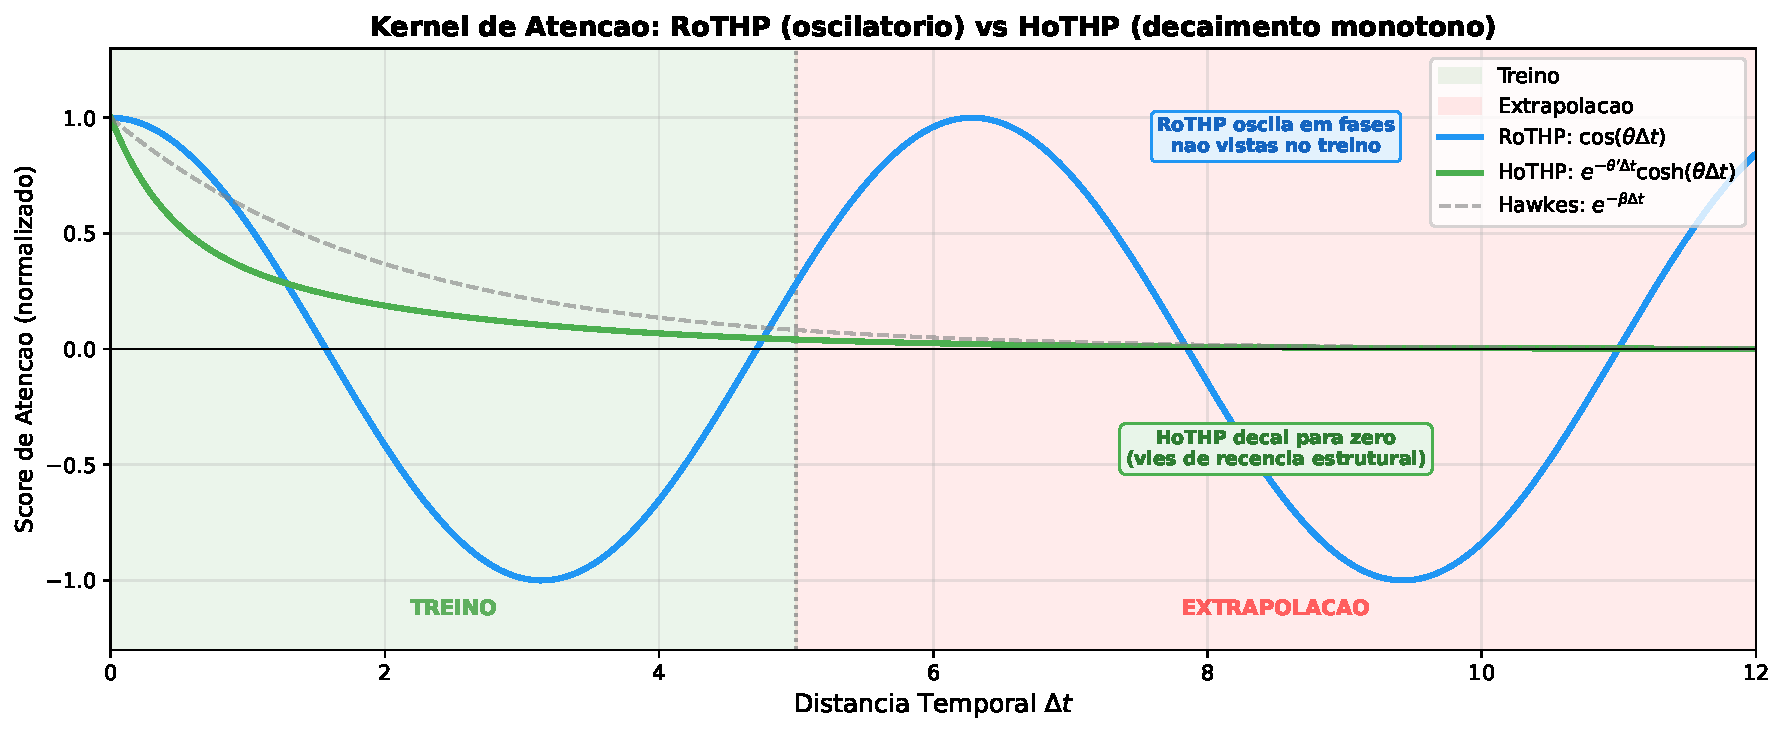
\includegraphics[width=14cm]{figuras/fig_kernel_rothp_vs_hothp.pdf}
    }{
    }
\end{figure}

% ---------------------------------------------------------------
\section{Configuração experimental}
\label{sec:configuracao-experimental}
% ---------------------------------------------------------------

Os experimentos usam dados sintéticos gerados por processos de Hawkes com kernel exponencial. A escolha de dados sintéticos é deliberada. Como conhecemos o processo gerador, podemos verificar se o viés de recência do HoTHP de fato se alinha com o decaimento real dos dados, e se essa correspondência é o que sustenta a extrapolação. Em dados reais, onde o kernel gerador é desconhecido, essa verificação não seria possível.

\subsection{Geração de dados sintéticos}
\label{subsec:geracao-dados}

Geramos sequências de processos de Hawkes multivariados com $K = 2$ tipos de evento e kernel exponencial. Definimos dois cenários de geração para cobrir regimes distintos de dependência temporal.

No \textbf{cenário de decaimento lento}, o parâmetro $\beta$ é pequeno, de modo que a influência de eventos passados persiste por mais tempo e eventos distantes ainda afetam a intensidade presente.

No \textbf{cenário de decaimento rápido}, $\beta$ é grande e apenas eventos recentes têm influência relevante.

Para cada cenário, geramos 500 sequências de treinamento, 150 de validação e 200 de teste. A simulação usa o algoritmo de desbaste de Ogata (\textit{Ogata's thinning algorithm}) \cite{ogata_lewis_1981}, um método de rejeição exata para gerar realizações de processos pontuais com intensidade variável.

\subsection{Protocolo \textit{train short, test long}}
\label{subsec:train-short-test-long}

O protocolo \textit{train short, test long}, proposto por \citeonline{press_train_2021} para modelos de linguagem, treina o modelo em sequências curtas e o testa em sequências mais longas. Adaptamos o protocolo para processos pontuais usando o número de eventos como medida de comprimento.

Varremos comprimentos de treinamento $L \in \{10, 20, 50, 100\}$ e fatores de extrapolação $\{1\times, 2\times, 5\times, 10\times\}$, onde o fator indica quantas vezes a sequência de teste é mais longa do que a de treinamento. Com $L = 10$ e fator $10\times$, por exemplo, treinamos com sequências de 10 eventos e testamos com sequências de 100. Ao todo, a varredura produz 16 combinações de $(L, \mathrm{fator})$, avaliadas nos dois cenários de decaimento.

\subsection{Modelos comparados e implementação}
\label{subsec:modelos-comparados}

Comparamos o HoTHP com o RoTHP \cite{gao_rothp_2024}. O RoTHP é o baseline natural porque os dois modelos têm exatamente a mesma estrutura de encoder e a mesma função de intensidade; a única diferença é o kernel posicional. O THP original não entra na comparação porque sua sensibilidade a deslocamentos temporais já foi documentada por \citeonline{gao_rothp_2024}.

Ambos os modelos são implementados no framework EasyTPP \cite{xue_easytpp_2024}, com os mesmos hiperparâmetros: $d = 64$, $N_{\ell} = 2$ camadas, $H = 4$ cabeças de atenção, \textit{dropout} de $0{,}1$ e Adam com taxa de aprendizado $10^{-3}$.

\subsection{Métricas e avaliação estatística}
\label{subsec:metricas}

A métrica de avaliação é a verossimilhança logarítmica negativa (NLL), calculada sobre a sequência completa de teste, incluindo os eventos além do comprimento de treinamento. O que nos interessa é a NLL na região extrapolada. Se o viés de recência do HoTHP de fato habilita a extrapolação, a NLL deve se manter estável mesmo quando a sequência de teste é muito mais longa do que a de treino.

Repetimos todos os experimentos com $N = 5$ sementes e reportamos média $\pm$ desvio padrão. Para verificar significância estatística, usamos o teste de Wilcoxon de postos sinalizados (\textit{Wilcoxon signed-rank test}), um teste não paramétrico pareado que não assume normalidade e é adequado para $N = 5$. Aplicamos o teste unilateral (hipótese alternativa: HoTHP $<$ RoTHP em NLL) com $\alpha = 0{,}05$.
